\chapter{Транспортные свойства и особенности кристаллической структуры соединений из группы тетраэдрита"--~теннантита (литературный обзор)} \label{chapt1}

Современное развитие техники предъявляет новые требования к функциональным материалам, задача поиска которых стоит перед наукой. Общепринятый способ получения термоэлектрических материалов заключается в модифицировании поликристаллических структур допированием атомами, которые повышают электропроводность. Другой способ~--- наноструктурирование материала, он используется для создания низкой теплопроводности с высоким значением электропроводности, возникающей за счёт проводящего межзёренного пространства. Третий способ создания термоэлектрических материалов основывается на наличии стеклоподобной теплопроводности за счёт наличия в кристаллической структуре обособленных комплексов атомов. Одними из таких перспективных функциональных материалов, обладающих стеклопододной теплопроводностью, являются соединения из группы тетраэдрита"--~теннантита с обшей структурной формулой (Cu\textsuperscript{+},Fe,Ag,Zn)\textsubscript{10}(Cu\textsuperscript{2+})\textsubscript{2}(As,Sb)\textsubscript{4}(S,Se)\textsubscript{13}.

Соединения группы тетраэдрита"--~теннантита также называют блеклыми рудами или сульфосолями. В минералогии эти соединения уже более 250 лет используются как индикаторы условий рудообразования. Кристаллическая структура соединений группы тетраэдрита"--~теннантита описывается кубической плотноупакованной решеткой с расположением катионов в лавесовских полиэдрах. Такая структура близка к сфалеритовой, но с параметром ячейки вдвое большим, чем у последней. Своё название эта структура получила благодаря тусклому блеску на изломе.

Соединения ряда тетраэдрит--теннантит, согласно принятой классификации в минералогии\cite{Molo2008}, относят к большой семье из подтипа сульфосолей класса халькогенидов, выделенных по химическим особенностям.
Понятие сульфосолей включает в себя широкий класс соединений (имеются ввиду минералы), содержащих трёхвалентные атомы As, Sb, Bi и, за редким исключением, четырехвалентный атом Te.
Подразумевается, что катионы As\textsuperscript{3+}, Sb\textsuperscript{3+}, Bi\textsuperscript{3+} и Te\textsuperscript{4+} связаны с катионом или катионами Me.
Причем анион  S\textsuperscript{2-} может быть заменён на Se\textsuperscript{2-} или Te\textsuperscript{2-}. Таким образом, общая зарядовая формула сульфосолей имеет следующий вид:

\begin{equation}
  \label{eq:equation1}
  (Me^+,Me^{'2+},etc.)_{x}[(Bi, Sb,As)^{3+}, Te^{4+}]_{y}[(S,Se,Te)^{(2-)}]_{z}.
\end{equation}

Важно отметить, что отличительной особенностью сульфосолей является электронное взаимодействие между катионами, например As\textsuperscript{3+}, Sb\textsuperscript{3+}, Bi\textsuperscript{3+} ввиду их ассиметричного расположения. Такая отличительная особенность структуры выделяет соединения с общей структурной формулой  \eqref{eq:equation1} в особую группу в классе халькогенидов. Данная классификация была введена по аналогии с существующей классификацией оксидов, как для (As\textsuperscript{3+}O\textsubscript{3})\textsuperscript{3$-$}, так и для (As\textsuperscript{5+}O\textsubscript{4})\textsuperscript{3$-$}\cite{Nowacki1969}.

В общем случае соединения ряда тетраэдрит--теннантит описываются структурной формулой:

\begin{equation}
  \label{eq:equation2}
      \begin{multlined}
      (Cu^{1+},Ag,Tl,Au)_{10}(Zn,Fe,Cu^{2+},Hg,Cd,Pb,Mn,Ni,Co,Sn)_{2}\times \\
      \times(As,Sb,Bi,Te,Ge,In)_{4}(S,Se)_{13}.
      \end{multlined}
\end{equation}
\newpage

%\newpage
%============================================================================================================================

\section{Структурные особенности соединений тетраэдрита и теннантита  и их связь с транспортными свойствами} \label{sect1_1}

 Структура тетраэдрита впервые была описана Полингом и Нейманом  \cite{Pauling1934} и уточнена в работах \cite{Wuensch1963,Wuensch1964,Belov1969,Kaplunnik1980}.
 В соврмененной литературе встречается два вида структурной формулы Cu(I)\textsubscript{6}Cu(II)\textsubscript{6}[(As,Sb)S\textsubscript{3}]S\textsubscript{4}\cite{Johnson1986} и Cu$_{10-x}^{+}$Cu$_{2+x}^{2+}$(As,Sb)$_{4}^{3+}$S$_{13}^{2-}$ \cite{Friese2008,makovicky2005crystal,Foit2001} (группа симметрии I$\overline{\! 4}$3m).
Данные соединения являются наиболее изученными, и их описания широко представлены в литературе. Структуры соединений тетраэдрита~--теннантита представляют собой тетраэдрические комплексы  CuVI\textsubscript{4}, где VI = S, Se, ориентированные в пространстве в одну сторону (Рис. \ref{img:figure1}а). Такое упорядочение тетраэдрических комплексов создаёт пустоты между ними, которые имеют форму усеченных тетраэдров (<<лавесовские полиэдры>>). <<Лавесовские полиэдры>> изображены на рисунке~\ref{img:figure1}б). В полученных усеченных тетраэдрах помещается по шесть атомов меди (Рис. \ref{img:figure1}в), каждый из которых окружен тремя атомами серы\cite{Makovicky_2006}. Ввиду ограниченного изоморфизма величина параметра элементарной ячейки изменяется от 10.16 до 10.33.

\begin{figure}[pt!]
  \begin{minipage}[ht]{0.99\linewidth}\centering
    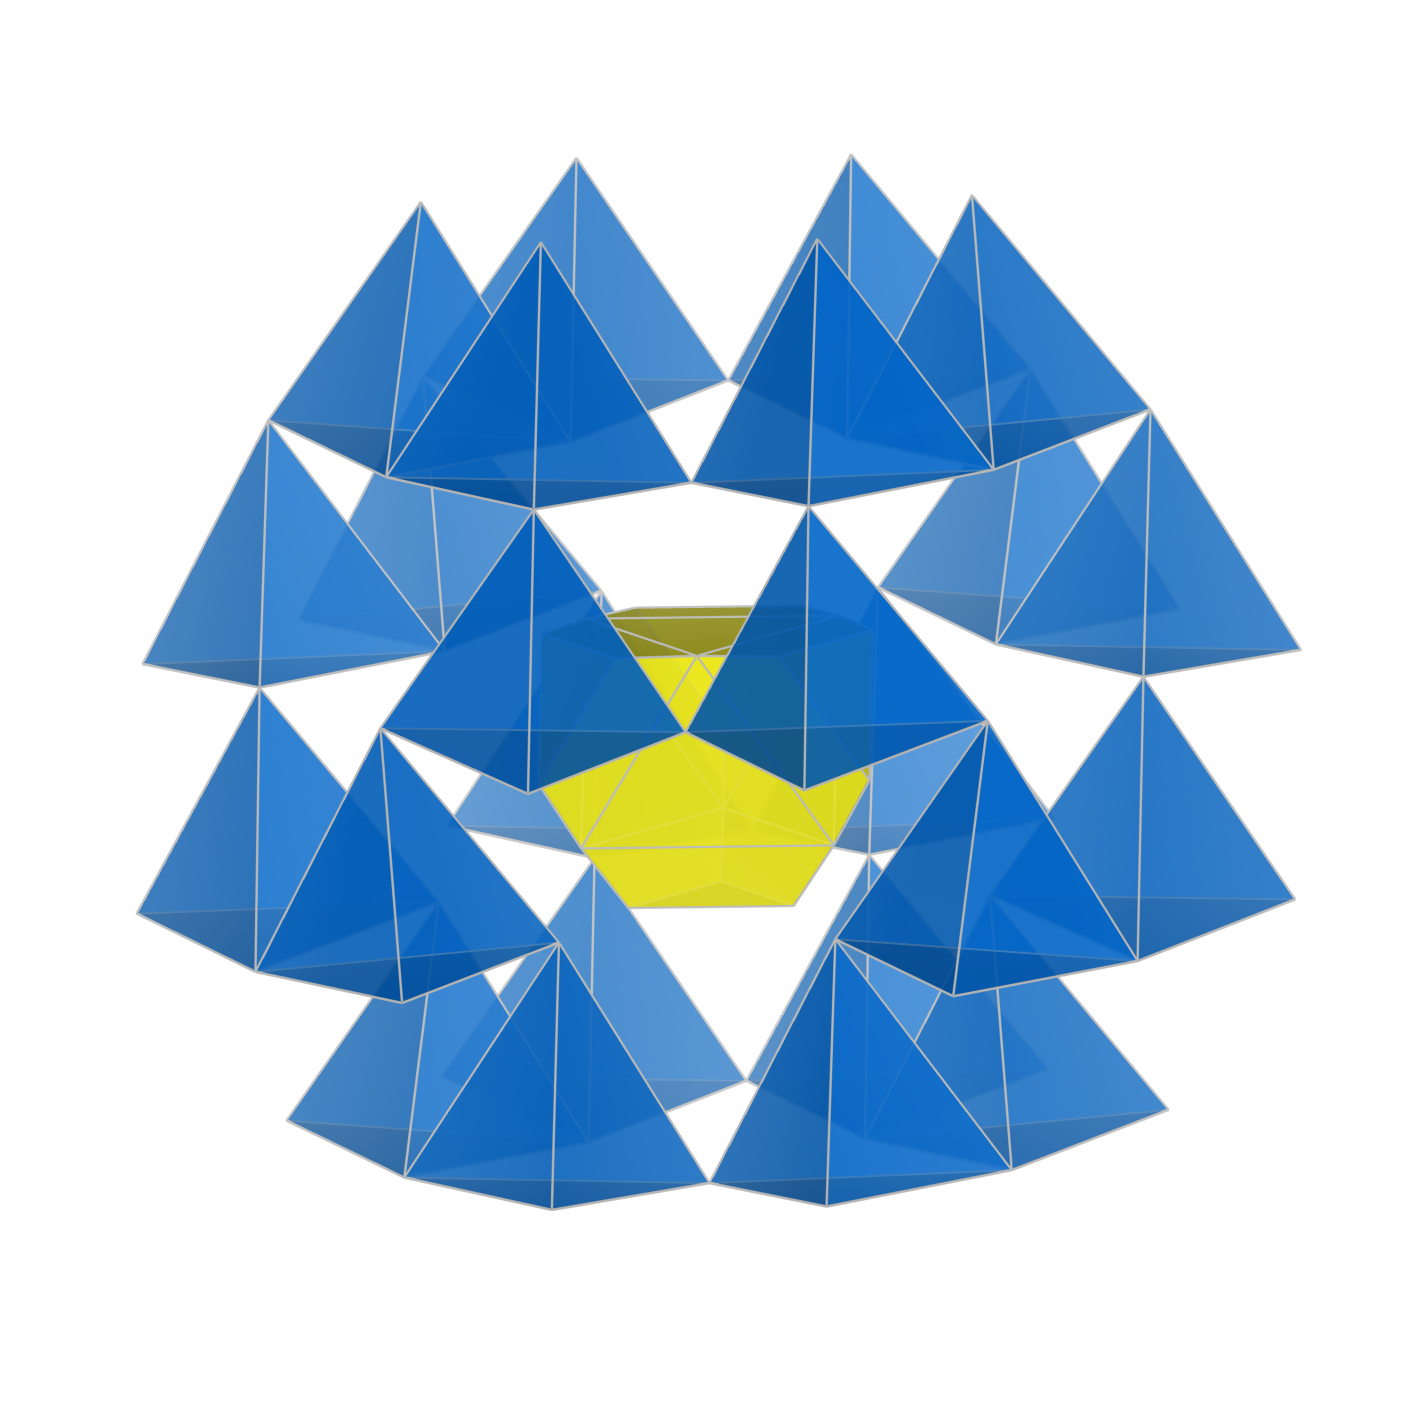
\includegraphics[width=0.6\linewidth]{2_cu12as4s13_crys_st_b} \\ а)
  \end{minipage}
  \vfill
  \begin{minipage}[ht]{0.99\linewidth}\centering
    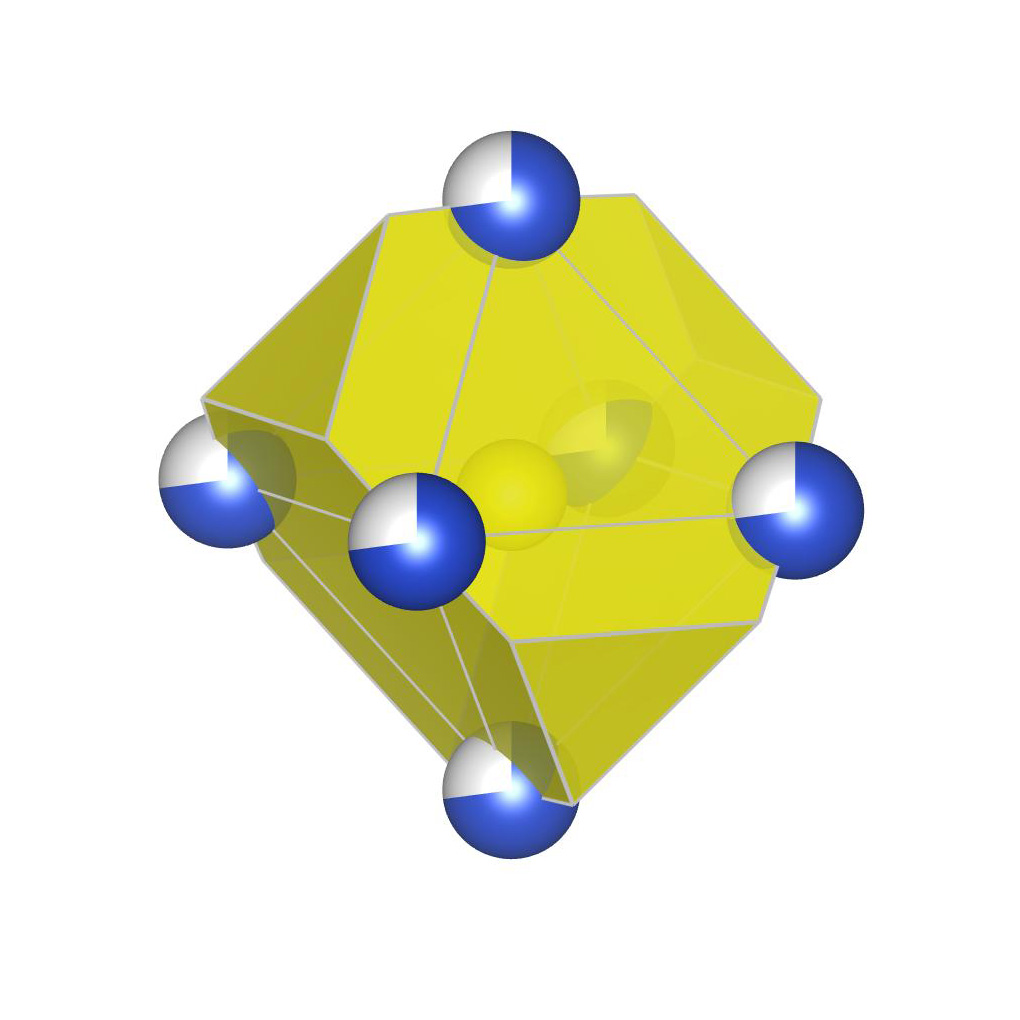
\includegraphics[width=0.6\linewidth]{3_cu12as4s13_crys_st_d} \\ б)
  \end{minipage}

      \caption[Кристаллическая структура халькогенида на примере синтетического теннантита Cu\textsubscript{12}As\textsubscript{4}S\textsubscript{13}]{Кристаллическая структура халькогенида на примере синтетического теннантита Cu\textsubscript{12}As\textsubscript{4}S\textsubscript{13}}
    \label{img:figure1}
\end{figure}

Структуры соединений тетраэдрита и теннантита являются близкими к структурам сфалерита или халькопирита\cite{Pauling1934}.
Если увеличить структуру сфалерита ZnS вдвое по ребру, то элементарная ячейка будет содержать в восемь раз больше атомов: 32 катиона Zn\textsuperscript{2+} и 32 аниона S\textsuperscript{2+}. И, заменяя часть металлических катионов Zn\textsuperscript{2+} катионами полуметалла X\textsuperscript{3+} и оставляя часть катионов одновалентными X\textsuperscript{+}, мы получаем состав A$^{+}_{24}$X$^{3+}_{8}$S$^{2-}_{32}$. Удаление восьми анионов S\textsuperscript{2-} создает характерные для тетраэдрита комплексы полуметаллов [X$^{3+}$S$^{2-}_{3}$]. Получившиеся дефекты образуют форму тетраэдров, соответствующую пустым октантам сфалеритовой ячейки. На месте восьми анионов S\textsuperscript{2-} находятся атомы полуметалла  X\textsuperscript{3+}, которые создают  неподелённые электронные пары. Таким образом, получается, что половина всех ионов A\textsuperscript{+} вблизи тетраэдров находится без полноценного окружения, координация по анионам S\textsuperscript{2-} равна двум, координация полуметаллов трём. Другая половина ионов A\textsuperscript{+} обладает четверной координацией, которая осталась как у сфалерита. Далее в центр из двух пустых тетраэдров обратной ориентации, где находятся неподелённые электронные пары, вводится дополнительный анион S\textsuperscript{2-}. Введение дополнительного аниона повышает S\textsuperscript{2-}  координацию половины атомов A\textsuperscript{+} до трех. После введения 2S\textsuperscript{2-} необходимо скомпенсировать заряд катионной части на четыре единицы, для чего четыре трёхкоординированных катиона A\textsuperscript{+} заменяются на A\textsuperscript{2+}. Получается, что общий состав тетраэдрита может быть выражен

\begin{equation}
  \label{eq:equation3}
  A^+_{20}A^{2+}_4[X^{3+}S^{2-}_{3}]^{3-}_{8}S_2.
\end{equation}



В литературе широко обсуждаются возможные методы построения структуры тетраэдрита. Авторы \cite{Koch_1981} рассматривают структуру тетраэдритов на основе кубически инвариантного комплекса  \textit{W*}. Этот комплекс находится около идеальных тетраэдров и обладает с ними общими вершинами.
Авторы статьи детально обсуждают соединения тетраэдрита и теннантита с точки зрения гомогенных или негомогенных структур в контексте W*(4t\textsubscript{c}) и (F$^{''}_{2}$-I(4t)) решеток.
Если рассматривается структура W*, то возможная максимальная симметричная группа для этой структуры~--- Im3m. В этом случае вершины располагаются в позиции 24(h) xx0 с $x = \frac{1}{4}\sqrt{2} = 0.3536$, центры этих вершин будут располагаться в 12(d) $\frac{1}{4}\frac{1}{2}0$.
В настоящее время таких структур не найдено, что оставляет открытым вопрос расположения атомов в элементарной ячейке тетраэдрита.
Также известно, что значение  z в позиции 24(g) xxz для силикатных структур лежит в диапазоне 0.025~$<$~z~$<$~0.085, в то время как этот же параметр для соединений со структурой тетраэдрита лежит в диапазоне 0.135~$<$~z~$<$~0.165.
Исходя из описанного выше, авторы приходят к мнению, что соединения из группы тетрадаэдрита и теннантита, относящиеся к I$\overline{\!4}$3m, могут быть описаны двумя разными гомогенными решетками W*(4t\textsubscript{c}) и (F$^{''}_{2}-$I(4t)), наследованными от силикатных структур.


Авторами работы \cite{Johnson1986} рассмотрено 1271 образцов натурального  и 295 синтетических образов тетраэдрита. Данная работа проведена с целью изучения механизмов замещения элементов Ag, Fe, Zn, Hg, Cd, As, Te, Bi в структуре тетраэдрита. Исследование показало, что на структурную формулу могут приходиться от четырех до десяти атомов Cu,  до четырех атомов Ag и не более двух атомов Fe, Zn, Hg. Возможно полное замещение между атомами As и Sb при неизменном составе атомов S в элементарной ячейке.
По данным авторов описать замещение атомами Pb, Bi и Cd не представлялось возможным ввиду малого количества данных. Структуры с замещенными атомами Co, Ni, Mn и Au не обнаружены. Предложена общая формула (Cu,Ag)\textsubscript{6}Cu\textsubscript{4}(Fe,Zn,Cu,Hg,Cd)\textsubscript{2}(As,Sb,Bi,Te)\textsubscript{4}(S,Se)\textsubscript{13}. Размер элементарной ячейки возрастает с увеличением атомного номера допируемых элементов, за исключением тетраэдритов содержащих Ag. Атомы Ag и As обладают низкой тенденцией к взаимодействию, что подтверждается графиками замещения для Fe от As, Zn от Ag, Hg от Cu. Для объяснения этих механизмов используется модель предложенная Джонсоном \cite{johnson1983brillouin}. Эта модель заключается в анализировании свободных электронов в структуре. Анализ показывает, что структура предсказывает наличие соединений со структурными формулами  Cu\textsubscript{14}Sb\textsubscript{4}S\textsubscript{13}~--- Cu\textsubscript{12}Sb\textsubscript{4.67}S\textsubscript{13}.

Этими же авторами \cite{Johnson1988} обсуждается кристаллохимия тетраэдритов, и предлагается общая формула \textsuperscript{IV}M(I)\textsubscript{6}\textsuperscript{III}M(II)\textsubscript{6}[\textsuperscript{III}X\textsuperscript{IV}Y\textsubscript{3}]\textsuperscript{VI}Z\textsubscript{4} (M(1) $=$ Cu, Fe, Zn, Mn, Hg, Cd; M(2) $=$ Cu, Ag; X $=$ Sb, As, Bi, Te; Y и Z $=$ S,Se)  для описания структуры тетраэдрита. Эта структура вводится по аналогии с содалитовой структурой с тетраэдрами M(1)Y\textsubscript{4}, которые содержат октаэдры ZM(2)\textsubscript{6}. Такое описание структуры приводит к увеличение связей между M(1)--Y и X--Y. Искажение решетки тетраэдра обуславливается влиянием изменения длины связи M(1)--Y и более сильным влиянием от изменения связи X--Y. Также отмечается влияние температуры и давления при синтезировании на кристаллографические особенности соединений. В заключении работы авторы делают вывод, что предложенная модель имеет ограничения при построении диаграммы P--T--X и необходимы дальнейшие исследования.

Вариации строения кристаллической структуры и полиморфизм в системе Cu--Sb--S при температуре ниже 400\textsuperscript{$\circ$}С рассматривается в исследовании \cite{Tatsuka_1977}. Основной результат работы заключается том, что тэтраэдрит стабилен при температуре 95\textsuperscript{$\circ$}С со структурной формулой Cu\textsubscript{12+x}Sb\textsubscript{4+y}S\textsubscript{13}, где 0.11~$\leqslant$~X~$\leqslant$~1.77 и 0.03~$\leqslant$~Y~$\leqslant$~0.3. Авторы установили, что ниже 95\textsuperscript{$\circ$}С соединение тетраэдрита образует две несмешиваемых фазы, которые описываются структурой тетраэдрита. Образование фаз быстрое и обратимое. Исследования структуры получившихся фаз показывают, что различие структуры двух фаз заключается в особенностях распределений позиций меди. Трансформация из одной фазы в другую происходит даже при добавлении лишнего атома меди или серы, в том числе и при комнатной температуре. Отмечается, что при комнатной температуре могут обнаруживаться фазы со структурными формулами Cu\textsubscript{12}Sb\textsubscript{4}S\textsubscript{13} и Cu\textsubscript{14}Sb\textsubscript{4}S\textsubscript{13}. Две эти фазы образуются на основе Cu\textsubscript{3}Sb\textsubscript{0,99}S\textsubscript{3}, с параметром ячейки a~$=$~20.848~$\pm$~0.006~$\angstrom$ и имеют название псевдотетраэдрит. Фаза псевдотетраэдрита стабильна до 350\textsuperscript{$\circ$}С и при более высокой температуре трансформируется в фазы тетраэдрита. Выше температуры 361\textsuperscript{$\circ$}С появляется высокотемпературная фаза Cu\textsubscript{3}SbS\textsubscript{3}. Превращение из фазы Cu\textsubscript{12}Sb\textsubscript{4}S\textsubscript{13} в Cu\textsubscript{14}Sb\textsubscript{4}S\textsubscript{13} и обратно объясняется мобильностью атомов меди в структуре.

На особенности формирования фаз система Cu--As--S исследовалась методами дифференциального термического и рентгенофазового анализов в работе \cite{Kurz_1989}. Установлено наличие квазибинарных соединений Cu\textsubscript{2}S--As, As--Cu\textsubscript{3}AsS\textsubscript{3}, Cu\textsubscript{3}S--Cu\textsubscript{2}S и Cu\textsubscript{2}S--As\textsubscript{2}S\textsubscript{3}. Также обнаружено два близких соединения Cu\textsubscript{6}As\textsubscript{4}S\textsubscript{9} и Cu\textsubscript{4}As\textsubscript{2}S\textsubscript{5}. Данные соединения и Cu\textsubscript{24}As\textsubscript{12}S\textsubscript{31} относятся к структуре производной от сфалеритовой, и находятся в области гомогенности соединения Cu\textsubscript{4}As\textsubscript{2}S\textsubscript{5} на фазовой диаграмме для системы  Cu--As--S. Отмечается наличие двух модификаций для соединения Cu\textsubscript{3}AsS\textsubscript{3}, низкотемпературная фаза которого известна как теннантит. Высокотемпературная фаза получается закалкой. Некоторые данные показывают, что соединения Cu\textsubscript{5}AsS\textsubscript{4} подобны минералу стефаниту Ag\textsubscript{5}SbS\textsubscript{4}. Соединения получены спеканием в кварцевых ампулах в вакууме. Часть структурных исследований была проведена на монокристальном дифрактометре Enraf--Nonius CAD 4. В работе детально описываются особенности получения описанных выше фаз.

В статье \cite{Makovicky1995} обсуждается полиморфная фаза Cu\textsubscript{3}SbS\textsubscript{3}. Автором предложена модель  структуры в триклинной сингонии (группа симметрии P2\textsubscript{1}/c). Параметры ячейки a~$=$~7.814(1)~$\angstrom$, b~$=$~10.242(1)~$\angstrom$, c~$=$~13.273(1)~$\angstrom$, $\beta$~$=$~90.29(1)\textsuperscript{$\circ$} c Z~$=$~8. Атом Sb находится в треугольной пирамидальной координации в окружении призм, созданных вследствие двойникования из-за ряда атомов~S ((11$\overline{\!2}$2)\textsubscript{hcp}). Длина связи Sb--S лежит в диапазоне от 2.26 до 2.47~$\angstrom$. Большинство атомов в позиции Cu обладают тройной координацией с длиной связи для Cu--S в диапазоне от 2.26 до 2.31~$\angstrom$. Позиция Cu4 обладает тройной или четверной координацией с длиной связи для Cu--S в диапазоне от 2.40 до 2.46~$\angstrom$. Отмечается, что P2\textsubscript{1}/c--скиннерит является низкотемпературной модификацией Cu\textsubscript{3}SbS\textsubscript{3}. Разница в особенностях расположения атомов меди в структурах P2\textsubscript{1}/c--скиннерит и P2\textsubscript{1}2\textsubscript{1}2\textsubscript{1}/c--виттихенит связывается с различным размером полиэдров Sb и Bi соответсвенно. 

Авторами \cite{Pfitzner1998a} продолжена классификация фаз соединения Cu\textsubscript{3}SbS\textsubscript{3}. Определена кристаллическая структура $\alpha$--Cu\textsubscript{3}SbS\textsubscript{3} при 493 К и 403 К методами монокристальной дифрактометрии. Высокотемпературная фаза, которая стабильна при температурах выше 394~К, кристаллизуется в орторомбическую кристаллическую решётку: параметры ячейки a~$=$~7.808(1)~$\angstrom$, b~$=$~10.252(2)~$\angstrom$, c~$=$~6.587(2)~$\angstrom$,  c Z~$=$~4, группа симметрии P\textsubscript{nma} (номер 62). Для данного соединения определено распределение атомов меди в тетраэдре [SbS\textsubscript{3}]\textsuperscript{3-}.  Атомы меди располагаются между пятью позициями с тройной или четверной координацией и пустых октаэдров S\textsubscript{6}.  Методами порошковой дифрактометрии при температуре 223~K определена кристаллическая структура $\gamma$--Cu\textsubscript{3}SbS\textsubscript{3}. Низкотемпературная фаза кристаллизуется в орторомбическую кристаллическую решётку: параметры ячейки a~$=$~7.884(1)~$\angstrom$, b~$=$~10.221(1)~$\angstrom$, c~$=$~6.624(1)~$\angstrom$,  c Z~$=$~4, группа симметрии P2\textsubscript{1}2\textsubscript{1}2\textsubscript{1}. Исследованные образцы получены спеканием в эвакуированных ампулах из соединений Cu\textsubscript{2}S и Sb\textsubscript{2}S\textsubscript{3} при температуре 853~К. Методика получения описана в работе \cite{Pfitzner_1994}. Отмечается, что структура высокотемпературной фазы определена на образце,  который использовался для определения структуры фазы $\beta$--Cu\textsubscript{3}SbS\textsubscript{3}. Обработка данных с монокристального эксперимента проводилась в JANA96, а с порошкового~---~в FULLPROF. Авторы отмечают, что структура для $\gamma$--Cu\textsubscript{3}SbS\textsubscript{3} получена методом Ритвельда с начальной структурой Cu\textsubscript{3}BiS\textsubscript{3}. Размер параметра кристаллической решетки для Cu\textsubscript{12}Sb\textsubscript{4}S\textsubscript{13} при температуре 223~К брался для определения особенностей структуры Cu\textsubscript{12+x}Sb\textsubscript{4}S\textsubscript{13}. Далее авторы проводят рассуждения о возможных вариантах расположения атомов меди в структуре, основываясь на  функции распределения электронной плотности. Атомы меди в позиции Cu(1) и Cu(2) находятся вне октаэдров S\textsubscript{6}. Атом меди в позиции Cu(3) располагается на гранях октаэдра  S\textsubscript{6}. Отмечается, что расстояние между атомами в позиции Cu(1) и Cu(2)~---2.099(9)~$\angstrom$, между  Cu(1) и Cu(3)~---1.266(9)~$\angstrom$, а между Cu(2) и Cu(3)~---1.93(1)~$\angstrom$. Полученные данные говорят о возможном нахождении атомов меди во всех трех позициях Cu(1), Cu(2) и Cu(3). Также авторы замечают, что структура Cu\textsubscript{3}SbS\textsubscript{3} не может быть описана в моноклинной сингонии. Высокотемпературная модификация имеет разориентировку как минимум вокруг пяти различных позиций, а уменьшение расстояния между атомами меди, необходимое для возникновения связи d\textsuperscript{10}--d\textsuperscript{10} оболочек с помощью введения дополнительного атома меди и аниона, может привести к появлению сверхрешётки, но дальнейших данных по этому предположению в статье нет.


В работе \cite{Makovicky2005} представлено первое исследование структуры монокристаллического образца минерала теннантит. Формула теннантита по результатом исследования авторов является Cu\textsubscript{12.5}As\textsubscript{0.98}Sb\textsubscript{0.02}S\textsubscript{13}. Исследование проведено на образце с линейными размерами 108$\times$72$\times$54~мкм\textsuperscript{3} при комнатной температуре и Mo K\textsubscript{$\alpha$} излучении на дифрактометре Bruker SMART CCD. Расстояние между кристаллом и детектором было 3.85 см. Параметры ячейки определены по 1068 рефлексам (I~$>$~8$\sigma$\textsubscript{I}) с помощью программного обеспечения SMART и SAINT. Образец проиндицирован в кубической сингонии I$\overline{\!4}$3m с размером ребра кристаллической ячейки 10.1756(9)~$\angstrom$ c R--фактором 0.072. Авторы отмечают, что основная часть позиций атомов полностью заселена и являлась фиксированной при дальнейшем уточнении структуры. Обнаружено, что позиции меди Cu2A и Cu2B не полностью заселены, и установлена корреляция между фактором смещения и заселенностью атомов в этих позициях. Между двумя атомами в позиции Cu2B находится один атом в позиции Cu2A, такое расположение образует ярко выраженные эллипсоиды, расположенные вдоль линии, соединяющей Cu2A и Cu2B.  По мнению авторов, такое расположение атомов подтверждает возможное статистическое распределение и движение атомов меди  по этим позициям. Заселенность позиций атомов Cu2A и Cu2B составляет 75 и 17~\% соответственно. Таким образом, получается, что почти в каждой позиции Cu2A находится атом меди. Данные структурного и химического анализа показывают, что могут существовать ситуации, при которых два атома меди будут находиться в позиции  Cu2B. Авторы отмечают, что проводили уточнение структуры в группе симметрии P1 и утроенной элементарной ячейки, и получили тот же результат, что и при уточнении в кубической симметрии. Рассуждения о частичной заселенности показывают, что в структуре не может находится вакантных позиций в лавесовском полиэдре.



В работе \cite{Nasonova2016} исследована структура низкотемпературной фазы синтетического тетраэдрита Cu\textsubscript{12}Sb\textsubscript{4}S\textsubscript{13}. Структура соединения получена методами порошкового рентгенофазового анализа в диапазоне температур от 10 до 293 К. Установлено, что при температуре около 90 К происходит фазовый переход типа металл--полупроводник,  смещение атома серы вдоль поверхности октаэдра Cu\textsubscript{6} и сдвиг атома меди вдоль треугольника S\textsubscript{3}, которые связаны с двумя независимыми позициями атомов серы и резким увеличением расстояния между Cu--Sb. Отмечается, что фазовый переход значительно влияет на транспортные свойства соединения: зарегистрировано резкое возрастание электрического сопротивления. Предположение о предсказании сверхструктуры не подтверждено \cite{Tanaka2015}.
Низкая теплопроводность, по мнению авторов, является следствием наличия квазилокализованных атомов меди, которые приводят к размягчению кристаллической решетки с повышением температуры.
Исследуемые образцы синтетического тетраэдрита были получены стандартным ампульным методом в стехиометрическом соотношении 12:4:13 в кварцевых ампулах под давлением 2$\times$10\textsuperscript{-2}~Торр. Ампулы нагревались до 973~К и отжигались в течение трех часов при этой температуре, после медленно охлаждались до 823~К в течение 30 часов, остывали при выключенной печи до комнатной температуры. Полученные спёки перетерались в агатовой ступке и были спресованы в таблетки под давлением 80--100~бар при комнатной температуре. Полученные таблетки отжигались в вакуумированных ампулах при 773~К в течение 25~часов. Структурные исследования были проведены на канале ID22 Европейского синхротронного источника с энергией $\lambda$~=~0.41066~$\angstrom$, с шагом 10~К в диапазоне температур от 10 до 150~К и с шагом 15~К в диапазоне температур от 150 до 240~К. Авторы отмечают, что все позиции атомов серы в соединениях Cu\textsubscript{12}Sb\textsubscript{4}S\textsubscript{13} и Cu\textsubscript{12}Sb\textsubscript{4}S\textsubscript{12.8} полностью заселены, за исключением позиции Cu(2). Для этих соединений установлены различные коэффициенты атомарных смещений 0.0102(4) и 0.0125(3) для позиции атома S(1), 0.016(2) и 0.019(2) для позиций атома S(2) и размер ребра элементарной ячейки 10.33051(2) и 10.33344(1)~$\angstrom$ соответсвенно для Cu\textsubscript{12}Sb\textsubscript{4}S\textsubscript{13} и Cu\textsubscript{12}Sb\textsubscript{4}S\textsubscript{12.8}. Ввиду близкого расположения позиций атомов Cu(2) для уточнения структуры при низких температурах взята структура Cu\textsubscript{12}Sb\textsubscript{4}S\textsubscript{13}  при комнатной температуре. С понижением температуры до фазового перехода кристаллическая ячейка уменьшается, но после фазового перехода размер кристаллической ячейки перестает уменьшаться с понижением температуры и показывает локальный максимум при 40~К. Этот фазовый переход вызван изменением положения атомов в позиции Cu(2). Так, максимальное и минимальное расстояние между позициями атома Cu(2) изменяется в три раза, а максимальное расстояния между позициями атомов Cu(2) и Sb(1) возникает при температуре соответствующей локальному максимуму размера кристаллической ячейки при 40~К. Ниже температуры фазового перехода возникает волна зарядовой плотности (или упорядочение зарядов Cu\textsuperscript{$+$}Cu\textsuperscript{$2+$} на атомах меди) за счет изменения позиций атомов меди Cu(2). Авторами исследованы транспортные свойства полученных соединений. Благодаря полученным ими данным была найдена характеристическая температура Дебая, возникающая ввиду наличия квазилокализованных фононных мод в кристаллической решетке. Авторы отмечают, что полученные ими данные для характеристических температур Эйнштейна отличаются от опубликованных в литературе данных\cite{Lara-Curzio2014}.

В работе \cite{Friese2008} проведено исследование синтетических тетраэдрита и теннантита, доппированного железом при температурах 25 и 250\textsuperscript{$\circ$}С. Исследованные соединения обладают структурной формулой Cu\textsubscript{12-x}Fe\textsubscript{x}(As,Sb)\textsubscript{4}S\textsubscript{13}, где  x~$=$~0.10 и 1.23 для теннантита  и  x~$=$~0.61 и 1.83~Fe для тетраэдрита.
 Увеличение количества атомов железа в структуре и теннантита, и тетраэдрита приводят к увеличению расстояния между Cu1--S и Cu2--S, где Cu1~---~позиция замещения для атома Fe. Позиция Cu2 определена как сдвоенная позиция. Расстояние Cu2--Cu2 составляет 0.56 и 0.65~$\angstrom$ для тетраэдрита и теннантита соответсвенно. С увеличением температуры параметр ребра кристаллической решетки увеличивается на 0.02--0.04~$\angstrom$, а в среднем межатомное расстояние увеличивается на 0.01~$\angstrom$. Полученное значение коэффициентов термического расширения для доппированных соединений такое жк, как и для недоппированных.
 В работе авторы детально обсуждают особенности распределения меди. Отмечается, что наблюдается смещение центра позиции Cu2 с повышением температуры. Расстояние Cu2--Cu2 в доппированных соединениях принимает типичное для сульфосолей расстояние при температуре 250\textsuperscript{$\circ$}С. Особенности распределения меди в тетраэдрите и теннантите разные:
межплоскостная плотность в теннантите выше, чем в тетраэдрите. Определенная разница в кристаллографических особенностях для исследованных образцов объясняется уменьшением зарядовой плотности в лавесовском полиэдре.
\newpage

\section{Структурные особенности соединений Cu\textsubscript{3}AsSe\textsubscript{3} и Cu\textsubscript{3}SbSe\textsubscript{3}} \label{sect1_2}

Данные о кристаллической структуре Cu\textsubscript{3}AsSe\textsubscript{3} и Cu\textsubscript{3}SbSe\textsubscript{3} в литературе немногочисленны.

Впервые минерал мгриит (Cu, Fe)\textsubscript{3}AsSe\textsubscript{3} описан в работе \cite{Dymlcov_1983}. Исследуемый образец представлял из себя шлиф породы, в котором обнаружены вкрапления исследуемой фазы. Твердость исследуемого образца лежит в диапазоне от 287 до 379~кг/мм\textsuperscript{2}. Измерения проведены на ПМТ--3 при нагрузке 20~г, времени 15~c и количестве измерений равным 33. Для сравнения: твердость теннантита лежит в диапазоне от 350 до 425~кг/мм\textsuperscript{2}. Количественный элементный анализ показывает формулу Cu\textsubscript{2.92}Fe\textsubscript{0.16}As\textsubscript{0.98}Se\textsubscript{2.96}. Рентгеноструктурный анализ проведен на характеристическом излучении Fe k\textsubscript{$\alpha$} на образцах диаметром 0.2 и 0.3~мм. Соединение обладает кубической сингонией и относится к группе симметрии Pd3M с параметром решетки a~$=$5.530$\pm$0.005~$\angstrom$, V~$=$169.48$\pm$0.005~$\angstrom^{3}$. Расчётная плотность составляет 4.9~г/см$^{3}$. Образец был предоставлен минералогическим музеем имени А. Е. Ферсмана.

В работе \cite{Majid_1987} рассматриваются трёхкомпонентные соединения, которые образуются в системе Cu--As\textsubscript{2}Se\textsubscript{3}. Основные результаты представлены в таблице \ref{tbl2}. Все соединения проиндицированы в кубической сингонии. Исследуемые образцы получены из особо чистых компонентов в стехиометрическом соотношении ампульным методом.

\begin{table} [htbp]%
    \centering
	\caption{Сводная таблица кристаллических фаз, образованных в системе Cu--As\textsubscript{2}Se\textsubscript{3}\cite{Majid_1987}}%
	\label{tbl2}% label всегда желательно идти после caption
    \renewcommand{\arraystretch}{1.5}
	\begin{tabular}{@{}@{\extracolsep{20pt}}llll@{}}
        \toprule     %%% верхняя линейка
    	Соединение& Параметр эл. яч., $\angstrom$&Объем эл. яч., $\angstrom^{3}$& Плотность, г/см\textsuperscript{3}	\\
        \midrule
    	Cu\textsubscript{3}AsSe\textsubscript{2} 	& 5.513$\pm$0.004	 & 167.47												&5.88	\\ \hline
    	Cu\textsubscript{3}AsSe\textsubscript{4} 	& 5.530$\pm$0.005	 						& 169.11												&5.75		\\ \hline
    	Cu\textsubscript{3}AsSe\textsubscript{3} 	& 5.758$\pm$0.009	 						& 190.87												&4.45		\\ \hline

        \bottomrule
	\end{tabular}%
\end{table}

Авторы статей \cite{39_Demb_1970,40_Demb_1971} опубликовали исследование твердых растворов в системе Cu\textsubscript{2}Se\textsubscript{3}--As\textsubscript{2}Se\textsubscript{3}. Отмечается, что в исследуемых твёрдых растворах при температуре 733~К образуется соединение Cu\textsubscript{3}AsSe\textsubscript{3}. Предполагается, что структура соединения обладает тетрагональной симметрией.
В работе \cite{39_Demb_1970} подробнее исследовалась система Cu\textsubscript{2}Se\textsubscript{3}--As\textsubscript{2}Se\textsubscript{3}. Результаты исследования показывают, что соединение Cu\textsubscript{3}AsSe\textsubscript{3} существует в интервале температур от 696 до 769~К, и реакция эвтектического распада медленно происходит  при температуре 393~К. Авторы работы \cite{bab_1982} проиндицированы соединение Cu\textsubscript{3}AsSe\textsubscript{3} в кубической сингонии с параметром решетки a~$=$10.11$\pm$0.01~$\angstrom$.


В работе \cite{31_Whitfield_1980} описано соединение Cu\textsubscript{3}SbSe\textsubscript{3}. Исследуемый образец получен спеканием соединений Cu\textsubscript{2}Se и Sb\textsubscript{2}S\textsubscript{3} в стехиометрических пропорциях ампульным методом при температуре 720~К в течение 48~часов. После обжига полученный образец был закалён в воде со льдом. Соединение обладает ромбической структурой и пространственной группой P\textsubscript{nma} с параметрами элементарной ячейки a~$=$7.97~$\angstrom$, b~$=$10.61~$\angstrom$ и c~$=$6.83~$\angstrom$, которая аналогична структурам соединений,  Cu\textsubscript{3}SbS\textsubscript{3} и  Cu\textsubscript{3}BiS\textsubscript{3}.


Отдельно стоит отметить, что широко обсуждаются механизмы и условия синтеза сложных халькогенидов. Основные результаты представлены в работах \cite{Sis_Frost2002,sis_karup59new,sis_Mueller2002,sis_Mueller2003,sis_Raghavan2004,sis_seal1990tetrahedrite,sis_Skinner1972,sis_Taras_Bryndzia_1988,sis_Tomkins2006,sis1_1347-4065-8-4-443,sis1_BALAZ1995375,sis1_Braga2008,sis1_Pfitzner:se0205,sis1_WELLER2017794}.
\newpage


\section{Физические свойства трёхкомпонентных соединений меди} \label{sect1_3}

Термоэлектрические и магнитные свойства в сложных халькогенидах связываются с особенностью распределения меди в <<лавесовских полиэдрах>>  и разориентировкой тетраэдрических комплексов в структуре. Так, например, аномально низкая теплопроводность связывается с ангармоническими тепловыми колебаниями в позиции атомов меди\cite{Mishra2017}, которые обуславливают возникновение аномально низкой теплопроводности. А изменение электронной структуры и, как следствие, изменение магнитных свойств, связываются с трансформацией комплексов  Cu\textsubscript{6}(S,Se)\textsubscript{12} при понижении температуры\cite{Gainov2008}. В тоже время опубликованные данные о механизмах формирования физических свойств различны, существует несколько мнений о механизмах низкотемпературных фазовых превращениях и в опубликованных данных не прослеживается общих трендов.


В статье \cite{Lai_2015} обсуждается связь влияния особенностей распределения меди в кристаллической структуре тетраэдрита Cu\textsubscript{12}Sb\textsubscript{4}S\textsubscript{13} или (Cu12d)\textsubscript{12}(Cu12e)\textsubscript{12}(Sb8c)\textsubscript{8}(S2a)\textsubscript{2}(S24g)\textsubscript{24} на его транспортные свойства. Авторы статьи показывают связь между локальной асимметрией связей  с термоэлектрическими свойствами.  
По мнению авторов, локальная асимметрия связей создаёт дополнительные связи, которые выявлены в пятиатомной структуре Sb[CuS\textsubscript{3}]Sb. Такие ассиметричные связи способствуют появлению мод, которые квазилокализованы и ангармоничны и обладают низкой фононной частотой и большой амплитудой. Подобные связи объясняют природу низкой теплопроводности в тетраэдритах. Авторы отмечают, что энергия таких мод составляет $\approx$~4 мэВ или соответсвует 33~см\textsuperscript{-1}.

Авторы работы \cite{Lara-Curzio2014} рассматривают особенности теплоёмкости в натуральных и синтетических образцах тэтраэдритов. Теплоёмкость природных  Cu\textsubscript{12$-$x}(Fe,Zn,Ag)\textsubscript{x}(Sb,As)\textsubscript{4}S\textsubscript{13} и синтетических Cu\textsubscript{12$-$x}Zn\textsubscript{x}(Sb,As)\textsubscript{4}S\textsubscript{13}, при x~$=$~0,1,2, образцов измерена в диапазоне от 2 до 380~К. Установлено, что полученные зависимости теплоёмкости хорошо описываются моделью Дебая с тремя дополнительными осцилляторами Эйнштейна равными 12, 32.5 и 97~К соответсвенно. Предполагается, что осцилляторы Эйнштейна появляются ввиду ангармонических тепловых колебаний атомов. Эти колебания возникают при нестабильном перекрытии d-орибитали Cu c p-орбиталью S.
Наличие осцилляторов Эйнштейна, которые обуславливаются ангармоническими тепловыми колебаниями атомов, уменьшает теплопроводность и, как следствие, улучшает термоэлектрические свойства.

В работе \cite{Gainov2008} рассматриваются электрические и магнитные свойства природного теннантита. Исследование проведено методом ядерного квадрупольного резонанса и методом измерения намагниченности в СКВИД магнетрометре. Авторы исследовали перескакивание спинов между комплексами CuS\textsubscript{3} через S\textsubscript{2}. Анализ полученных зависимостей показывает наличие фазового магнитного перехода около 65~К. Магнитная восприимчивость измерена в диапазоне от 2 до 300~К и имеет характерный вид для парамагнетика. Основной вклад в парамагнетизм внесен ионами Fe\textsuperscript{2+}. В обсуждении результатов отмечается высокая чувствительность метода к изоморфным аналогам. Авторы определили энергию активации, которая соответсвует 65~К. Ниже этой температуры происходит замерзание внутренних локальных флуктуаций, которые связываются с необычным поведением квадрупольной частоты меди. Авторами рассматривается вопрос о валентности атомов меди. Отмечается, что локальные флуктуационные поля от Cu\textsuperscript{1+} влияют на осцилляции Cu\textsuperscript{2+}, наиболее значимое влияние оказывает первая координационная сфера. Тогда получается, что Cu\textsuperscript{2+} находятся в кластере Cu\textsubscript{6}S\textsubscript{13}. Это предположение вводится по аналогии с данными из работы\cite{Pattrick1993}, где кластер [Fe\textsubscript{3}S\textsubscript{4}]\textsuperscript{0} сравнивается с Cu\textsubscript{6}S\textsubscript{13} и предполагается наличие обменного взаимодействия.  Также рассматриваются деформация кристаллической структуры и изменение локального электронного окружения в контексте наличия эффекта Яна--Теллера, связанного с  Cu\textsuperscript{2+}.

Авторы работы \cite{DiBenedetto2002} провели исследование 130  природных образцов тетраэдритов из Природного музея Флоренции методами электронного сканирующего микроскопа, рентгенофазового порошкового анализа, дифференциального термического анализа, электронного парамагнитного резонанса и методом СКВИД магнитометра. Исследования электронного парамагнитного резонанса и измерения магнитной восприимчивости проведено на выборочных образцах. Во всех образцах найдено небольшое количество Cu\textsuperscript{2+} и Fe\textsuperscript{2+}. Fe\textsuperscript{3+} обнаружен только в дефектных образцах. Исследования электронного парамагнитного резонанса на отобранных образцах с высокой концентрацией Cu\textsuperscript{2+} показывают сильную анизотропию. Для объяснения анизотропии рассматривается модель несвязанных электронов двух парамагнитных центров, которые почти полностью делокализованы в направлении Cu--S--Cu. В данном направлении образуются мосты, которые в основном образованы p- и d-орбиталями\cite{Albright_2013}. Также рассматриваются зависимости обратной магнитной восприимчивости от температуры с учетом высокотемпературной магнитной модели Гейзенберга. Отмечается наличие антиферромагнитных взаимодействий, а также двухвалентность атомов железа, которые находятся в позициях тетраэдров. Авторы делают вывод, что атомы Cu\textsuperscript{2+}, находятся в образцах, где сумма катионов меньше 12, координационный полиэдр Cu\textsuperscript{2+} разориентирован, наличие взаимодействия между Cu\textsuperscript{2+} говорит о наличии диммеров. Обнаружено наличие остаточной намагниченности при температурах ниже фазового перехода. При 4.2~К наблюдается наличие парамагнитных центров.  Измерения электронного парамагнитного резонанса проведены на спектрометрах Bruker~200D и Bruker~ESP380.

Продолжением предыдущей работы является статья \cite{DiBenedetto2005}, в которой исследуются магнитные свойства синтетического тетраэдрита Cu\textsubscript{12}Sb\textsubscript{4}S\textsubscript{13}. Синтетический тетраэдрит исследован методами измерения намагниченности, дифференциальной сканирующей калориметрии и импульсного электронного парамагнитного резонанса для получения данных о распределении атомов Cu\textsuperscript{2+}.
Сильное антиферромагнитное упорядочение, наблюдаемое при комнатной температуре, связано с фазовым переходом при 85~К. Авторами установлено, что атомы Cu\textsuperscript{2+} случайным образом расположены в позиции тетраэдрита M(1). По мнению авторов, такое расположение атомов меди в структуре создает антиферромагнитное взаимодействие. Тем не менее, ниже температуры Нееля наблюдаются парамагнитные ионы, которые расположены в межзёренном пространстве. Исследуемые образцы были получены синтезом из бинарных соединений CuS, Cu\textsubscript{2}S, Sb\textsubscript{2}S\textsubscript{3} в среде KCl:LiCl при температуре 400\textsuperscript{$\circ$}С. Образцы аттестованы методам порошкового рентгеноструктурного анализа и анализом на элементный состав. Магнитная восприимчивость измерена в диапазоне от 2 до 298~К на СКВИД магнитометре в режиме FC при постоянных магнитных полях 2 и 0.1~T. Теплоёмкость измерена на Quantum Design
PPMS в диапазоне температур от 75 до 100~К. В работе приводится литературный обзор по особенностям распределения меди в структуре тетраэдритов. График магнитной восприимчивости имеет отклонение в диапазоне температур от 60 до 100~К. Детальное исследование графика магнитной восприимчивости показывает, что фазовый переход лежит между 79~К и 86~К. График зависимости теплоёмкости имеет вид почти линейной зависимости в диапазоне от 85 до 100~К. Полученные зависимости электронного парамагнитного резонанса показывают, что несвязанные электроны Cu\textsuperscript{2+} взаимодействуют с большим количеством протонов и с ядром Sb. Авторы приходят к выводу, что особенности взаимодействия ионов Cu\textsuperscript{2+} определены. Также исследуются возможные причины возникновения неординарных магнитных свойств.



В работе \cite{Levinsky_2015} рассмотрены магнитные и термоэлектрические свойства четырех природных образцов из группы тетраэдрита--теннантита. Интерес к исследованию этих соединений вызван высоким потенциалом их использования как функциональных материалов для термоэлектрических устройств. Все образцы показывают p--тип проводимости с низкой мобильностью. Антиферромагнитное взаимодействие обуславливается наличием атомов Fe\textsuperscript{2+}. Максимальное значение ZT составляет 0.13 при температуре 700~K. Данное значение обусловленно высоким сопротивлением. Для измерения термоэлектрических свойств образцы были перетерты и дополнительно подготовлены методом плазменного спекания. Исследования магнитных свойств показывает, что  атомы железа в структуре могут находиться в качестве ферромагнитных атомов. Дальнейшие улучшение термоэлектрических свойств происходит за счет модифицирования реальной части сопротивления.

В работе \cite{Suekuni_2013} синтезированы  соединения Cu\textsubscript{12-x}Ni\textsubscript{x}Sb\textsubscript{4}S\textsubscript{13} (где x~$=$~0,~0.5,~1.0,~1.5 и 2.0), и проведено исследование термоэлектрических свойств. Авторы отмечают наличие низкоэнергетичных мод у атомов в позиции Cu(2) находящегося вне CuS\textsubscript{3}. Эти моды приводят к низкой теплопроводности ниже чем 0.5~В\textsuperscript{-1}м\textsuperscript{-1}. Допирование Ni приводит к возрастанию значения ZT. Максимальное значение 0.7 достигается при x~$=$~1.5 и температуре 665~К. Образцы были подготовлены ампульным методом. Шихты закладывались в стехиометрическом соотношении, нагревались в вакууме до температуры 973~К и выдерживались в течении 3 часов. Далее в течении 30 часов ампулы обжигались при температуре 823~К и остывали до комнатной температуры. Полученные образцы были измельчены и спрессованы в таблетки, которые обжигались в вакууме при температуре 773~К в течение 25 часов. Отожжённые образцы были повторно измельчены и спечены при температуре 803~К в течении одного часа в аргоне при давлении 60~МПа. Согласно данным рентгеноструктурного анализа атомы в позиции Cu(1) находились в тетраэдрах CuS\textsubscript{4}. Значение параметра кристаллической решетки лежало в диапазоне от 10.319--10.323$\angstrom$, что хорошо согласуется с опубликованными ранее данными. Авторы детально рассматривают величину значения тепловых колебаний атомов меди. По этой величине авторы определяют температуру Дебая, соответствующую этим колебаниям. Проведены оценки электропроводности по закону Видемана--Франца, из которых установлено, что наблюдается высокое рассеяние на фононах. Такое высокое рассеяние обуславливается наличием 58 атомов в элементарной ячейке и/или наличием низкоэнергетических мод ввиду особенностей распределения атомов меди. В заключение авторы отмечают, что высокое значение ZT обеспечивается низким значением решеточной теплопроводности.

Работа \cite{Suekuni2012} посвящена исследованию влияния допирования атомов Mn, Fe, Co, Ni, Cu и Zn на термоэлектрические и магнитные свойства в тетраэдрите Cu\textsubscript{12}M\textsubscript{2}Sb\textsubscript{4}S\textsubscript{13}.
Максимальное значение ZT достигается при M~$=$~Ni и составляет 0.15 при температуре 340~К.
Образцы получены стандартным ампульным методов в вакууме. Шихта в стехиометрическом соотношении нагревалась до 973~К, охлаждалась до 823~К в течение 30~часов, после~---охлаждалась вместе с печью до комнатной температуры.
Образцы получены с относительной плотностью 75--85~\%.
Сводные данные для соединений представлены ниже в таблице \ref{tbl1}.
В ходе рассуждений авторы приходят к выводу, что термоэлектрические свойства зависят не только от особенностей фононного рассеяния при внедрении атомов замещения, но также от изменения электронной структуры, которая меняется при допировании (атом замещения изменяет энергетическую щель вблизи энергии Ферми).
В заключение авторы отмечают, что термоэлектрические свойства соединения со структурой тетраэдрита чувствительны к допированию. Также эти соединения обладают низкой решеточной проводимостью, соединение синтетического тетраэдрита претерпевает фазовый переход металл--полупроводник при температуре 85~К и аномальный гистерезис при 300~К.


\begin{table} [htbp]%
    \centering
	\caption{Сводная таблица термоэлектрических свойств допированных соединений на основе тетраэдрита\cite{Suekuni2012}}%
	\label{tbl1}% label всегда желательно идти после caption
    \renewcommand{\arraystretch}{1.5}
	\begin{tabular}{@{}@{\extracolsep{20pt}}llll@{}}
        \toprule     %%% верхняя линейка
    	Атом замещения, M& $\angstrom$&мкВ/(K$^2$$\cdot$м)& ZT	\\
        \midrule
    	Mn 	& 10.42(1)	 						& 88												&0.07	\\ \hline
    	Fe		& 10.38(1) 	 						& 7													& 0.01		\\ \hline
    	Co		& 10.35(1) 						   & 37												& 0.03		\\ \hline
    	Ni		& 10.31(1) 							 & 177												& 0.15		\\ \hline
     Cu		& 10.31(1) 							 & 374												& 0.13		\\ \hline
		Zn		& 10.38(1) 							 & 46												& 0.03		\\ \hline
        \bottomrule
	\end{tabular}%
\end{table}


В работе \cite{Lu2013} исследуется влияние допирования в позиции меди в тетраэдрите Cu\textsubscript{12-x}M\textsubscript{x}Sb\textsubscript{4}S\textsubscript{13}, где атомами замещения служат атомы Zn или Fe. Соединения, исследованные в работе, получены стандартным ампульным методом, последующим отжигом и горячим прессованием. При значении x в диапазоне от 0 до 1.5 в соединении Cu\textsubscript{12-x}Zn\textsubscript{x}Sb\textsubscript{4}S\textsubscript{13} электропроводность в соединениях составляет 10\textsuperscript{-5}~Ом$\cdot$м. При значении x равном 1.5 сопротивление возрастает на один порядок в сравнении с оригинальным образцом.  При значении x равном 2 соединение становится изолятором. Различия обусловлены тем, что в работе \cite{Suekuni2012} в исследованных соединениях была примесь другой фазы. Допирование атомами Zn приводит к значительному возрастанию коэффициента Зеебека. Также авторами исследовано влияние допирования атомами Fe в соединении Cu\textsubscript{12-x}Fe\textsubscript{x}Sb\textsubscript{4}S\textsubscript{13}, где x~$=$~0.2,~0.5 и 0.7, на термоэлектрические свойства. Максимум значения ZT равное 0.8 достигается при x~$=$~0.5. Отмечается, что сопротивление Cu\textsubscript{11}Zn\textsubscript{4}S\textsubscript{13} в три раза больше, чем у Cu\textsubscript{11}FeSb\textsubscript{4}S\textsubscript{13}. Это обуславливается различием валентности между атомами Fe и Zn, которое приводит к изменению количества дырок в валентной области. Это позволяет авторам объяснить высокое значение коэффициента ZT равное 0.8.

В работе \cite{Heo2014} исследуются тепловые и электрические свойства синтетического тетраэдрита Cu\textsubscript{12}Tn\textsubscript{2}Sb\textsubscript{4}S\textsubscript{13}, где Tn~$=$~Mn, Fe, Co, Ni, Zn и твердого раствора Cu\textsubscript{12-x}Mn\textsubscript{x}Sb\textsubscript{4}S\textsubscript{13}, где 0~$\leq$~x~$\leq$~2. Исследование проводится для определения термоэлектрической эффективности каждого из соединений. По результатом экспериментов установлено, что соединение Cu\textsubscript{12}Sb\textsubscript{4}S\textsubscript{13} обладает самым высоким значением фактора мощности ввиду высокого значения электрической проводимости. Максимальное значение термоэлектрической эффективности из серии соединений Cu\textsubscript{12}Tn\textsubscript{2}Sb\textsubscript{4}S\textsubscript{13} получено для структуры, допированной Mn, и составляет 0.8 при 575~К. Добавление одного атома  Mn на структурную формулу Cu\textsubscript{12}Sb\textsubscript{4}S\textsubscript{13} приводит к значению термоэлектрической эффективности равной 1.13 при 575~К.

Также рассматриваются термоэлектрические свойства для твердых растворов Cu\textsubscript{12}Sb\textsubscript{4}S\textsubscript{13-x}Se\textsubscript{x}, где x~$=$~0,~0.5,~1.0 и 2.0\cite{Lu2016}.
Данная работа направлена на исследование замещения анионов в структуре тетраэдрита.
В работе приводятся расчёты методом теории функционала электронной плотности и проведено структурное исследование на линии 11BM  синхротронного источника третьего поколения в Аргоннской национальной лаборатории.
Расчёты показывают, что атом Se должен внедряться в позицию 24g тетраэдра.
Допирование атомами Se приводит к уменьшению электрического сопротивления без уменьшения значения ZT.
При x~$=$~1 наблюдается возрастание на 30~\% тепловой мощности в сравнении с Cu\textsubscript{12}Sb\textsubscript{4}S\textsubscript{13}.
Методика получения соединений описана ранее в работах \cite{Lu2013,Lu_2013b,Lu_2013}. По расчётам один допирующий атом Se  добавляет общую энергию 20~мэВ на кристаллическую ячейку, два~--- 30~мэВ.
Допирование третьим атомом Se делает структурную ячейку нейтрально заряженной. Расчёты также предсказывают отличное внедрение атома Se в позицию S(1) при комнатной температуре и выше. Авторы отмечают, что не учитывают возможность формирования стабильных соединений в систему Cu--Sb--Se.
Термоэлектрические свойства для всех образцов имеют одинаковый характер, который согласуется с опубликованными данными.
Как отмечено ранее, коэффициент ZT не изменяется несмотря на уменьшение сопротивления в образце.
Это связывается с добавлением  валентной зоны к уровню Ферми за счет допирования.
Такое добавление повышает перенос заряда в соединениях.
Увеличение электропроводности наблюдается для соединений с  x~$=$~2 выше температуры 600~K. Особенности увеличения электропроводности выше температуры 600~K подтверждается теоретическими расчётами и не обсуждается в работе.
Авторы же исследуют особенности влияния включения Cu\textsubscript{12}Sb\textsubscript{4}S\textsubscript{13} в твердый раствор.

Исследования ядерного магнитного резонанса, магнитной восприимчивости и проводимости синтетического тетраэдрита Cu\textsubscript{12}Sb\textsubscript{4}S\textsubscript{13} проведены\cite{Kitagawa2015} до давления 4 ГПа. Авторами отмечается, что при давлении выше 1 ГПа может возникать особое магнитное упорядочение. Анализ данных проведен в предположении наличия одно- и двухвалентных атомов меди.


В работе \cite{Kosaka2017} представлено исследование влияния допирования синтетического тетраэдрита. В неё исследовано замещение в Cu\textsubscript{12-x}M\textsubscript{x}Sb\textsubscript{4}S\textsubscript{13}, где атомами замещения служат атомы Mn, Fe, Co, Ni и Zn. Также исследовано влияние замещения на температуру фазового перехода металл-полупроводник. Авторы работы расширяют ряд допированных соединений образцами Cu\textsubscript{12-x}M\textsubscript{x}Sb\textsubscript{4}S\textsubscript{13}, где атомами замещения служат атомы Ge и Sn при x~$\leq $~0.6. Исследование авторов подтверждает, что фазовый переход предотвращается ввиду заполнения электронной оболочки меди, подтверждается внедрение допируемых атомов в <<лавесовский>> полиэдр. Внедрение четырёхвалентных атомов вместо одновалентной меди приводит к возрастанию термоэлектрической интенсивности и возникновению низкой теплопроводности материала. По результатам исследования максимальное значение термоэлектрической добротности составляет 0.65 при температуре 665~К, x~$=$~0.3~$-$~0.5 и при допировании Ge и Se.

Актуальный обзор статей, посвященных термоэлектрическим свойствам,  можно найти по ссылке \cite{Powella}. В работах \cite{ther_10.1007/s11664-016-4893-7,ther_10.1016/j.intermet.2016.08.003,ther_10.1016/j.jallcom.2017.01.187,ther_10.1039/C7RA02564E,ther_10.1039/C7TC00762K,ther_AENM:AENM201200650,ther_C5TC01636C,ther_C6DT00564K,ther_doi:10.1021/acs.chemmater.7b00891,ther_doi:10.1021/acs.inorgchem.7b02128,ther_doi:10.1021/acs.jpcc.7b02068,ther_doi.org/10.1016/j.jssc.2017.01.003,ther_GONCALVES2016209,ther_HARISH2016323,ther_JACE:JACE13838,ther_lu2014effect}  представлены исследования термодинамических свойств сложных халькогенидов при допировании и при разных условиях синтеза.
В работе \cite{Kehoe_2013} рассматривается возможность использования соединений Cu\textsubscript{3}MCh\textsubscript{3} (M~$=$~Sb, Bi; Ch~$=$~S, Se) в фотовольтаике. В работе проведено моделирование электрофизических свойств соединений.
Авторы отмечают, что данные соединение могут быть перспективным материалом для солнечных батарей. Отмечается, что ширина энергетической щели составляет 1.76, 1.79 и 1.43~эВ для Cu\textsubscript{3}SbSe\textsubscript{3}, Cu\textsubscript{3}BiS\textsubscript{3} и Cu\textsubscript{3}BiSe\textsubscript{3} соответсвенно. Все материалы относятся к непрямозонным полупроводникам. Сильный вклад в электрические свойства вносит обменное взаимодействие через атомы Sb и Bi.
\newpage
